\section{Experiments}
Here I presented a series of experiments on real-life dataset to find the best
classifiers to predict the publication conference. First I introduce my
dataset source and the cleaned data statistics. Then I showed the extracted
features. Next I explored several different classifiers to get the
best performance classifiers. At last, I would do parameter tuning for
optimization.


\subsection{Dataset}
I used the dataset from AMiner system, which is an academic social network
mining system \cite{tang2008arnetminer}. After cleaning, the whole dataset
contains over 1.5m papers. I filtered the papers in the top 10 most common
conference. The filtered dataset contains 10k publications from 10 conferences.
The dataset contains 31475 words, 5953 organizations, time ranging from 1978 to
2014. The dataset contains 14951 authors. However, most authors are sparse,
which means they would only appear once. This kind of author would not help much
in building upstream conditioning LDA model but cost much memory, therefore,
I filtered those sparse authors, and kept around 2k+ common authors for modeling.
I did similar filtering operations to organizations.



\subsection{Extracted Features}
I first presented our extracted features. Meta-data is just encoded via sparse
index matrix, with the document size times the meta-data size. Meta-data is
used as the input for Neural Networks Upstream Conditioning LDA.

\subsubsection{Topic Distributions}
I presented the topic-word distributions (top 10 words) of LDA and Neural
Networks Upstream Conditioning LDA. The above columns are the trained Upstream LDA,
and below column are the corresponding basic LDA:


% Topic 0 - Topic 4
\begin{minipage}{.196\textwidth}
\centering
\textbf{Algorithm} \\
algorithm \\
optimal \\
paper \\
set \\
based \\
graph \\
algorithms \\
proposed \\
size \\
methods
\end{minipage}
\begin{minipage}{.196\textwidth}
\centering
\textbf{Programing} \\
code \\
test \\
development \\
web \\
data \\
cost \\
cache \\
programing \\
software \\
testing
\end{minipage}
\begin{minipage}{.196\textwidth}
\centering
\textbf{Network} \\
network \\
power \\
leakage \\
energy \\
link \\
node \\
random \\
matrix \\
performance \\
communication
\end{minipage}
\begin{minipage}{.196\textwidth}
\centering
\textbf{Social} \\
social \\
human \\
link \\
clustering \\
opinion \\
society\\
network \\
user \\
algorithm \\
search
\end{minipage}
\begin{minipage}{.196\textwidth}
\centering
\textbf{Machine Learning} \\
data \\
svm \\
kernel \\
flow \\
algorithm \\
research \\
approach \\
simulation \\
environment \\
performances
\end{minipage}
% Topic 0 - Topic 4

% Topic 5 - Topic 9
\begin{minipage}{.196\textwidth}
\centering
algorithms \\
graph \\
set \\
time \\
tree \\
rate \\
paper \\
framework \\
solution \\
efficient
\end{minipage}
\begin{minipage}{.196\textwidth}
\centering
dynamic \\
computing \\
code \\
resources \\
programing \\
implementation \\
load \\
language \\
allows \\
words
\end{minipage}
\begin{minipage}{.196\textwidth}
\centering
network \\
networks \\
proposed \\
sensor \\
nodes \\
protocal \\
delay \\
layer \\
based \\
link
\end{minipage}
\begin{minipage}{.196\textwidth}
\centering
user \\
social \\
information \\
interaction \\
study \\
online \\
future \\
design \\
using \\
online
\end{minipage}
\begin{minipage}{.196\textwidth}
\centering
model \\
models \\
modeling \\
stucture \\
terms \\
svm \\
approach \\
research \\
study \\
global
\end{minipage}
% Topic 5 - Topic 9

From the top 10 words in typical Learned topics, we could see that the extracted
features are similar. Then I presented the training likelihood over iteration to
show the converge speed.

\begin{figure}[!htbp]
    \centering
    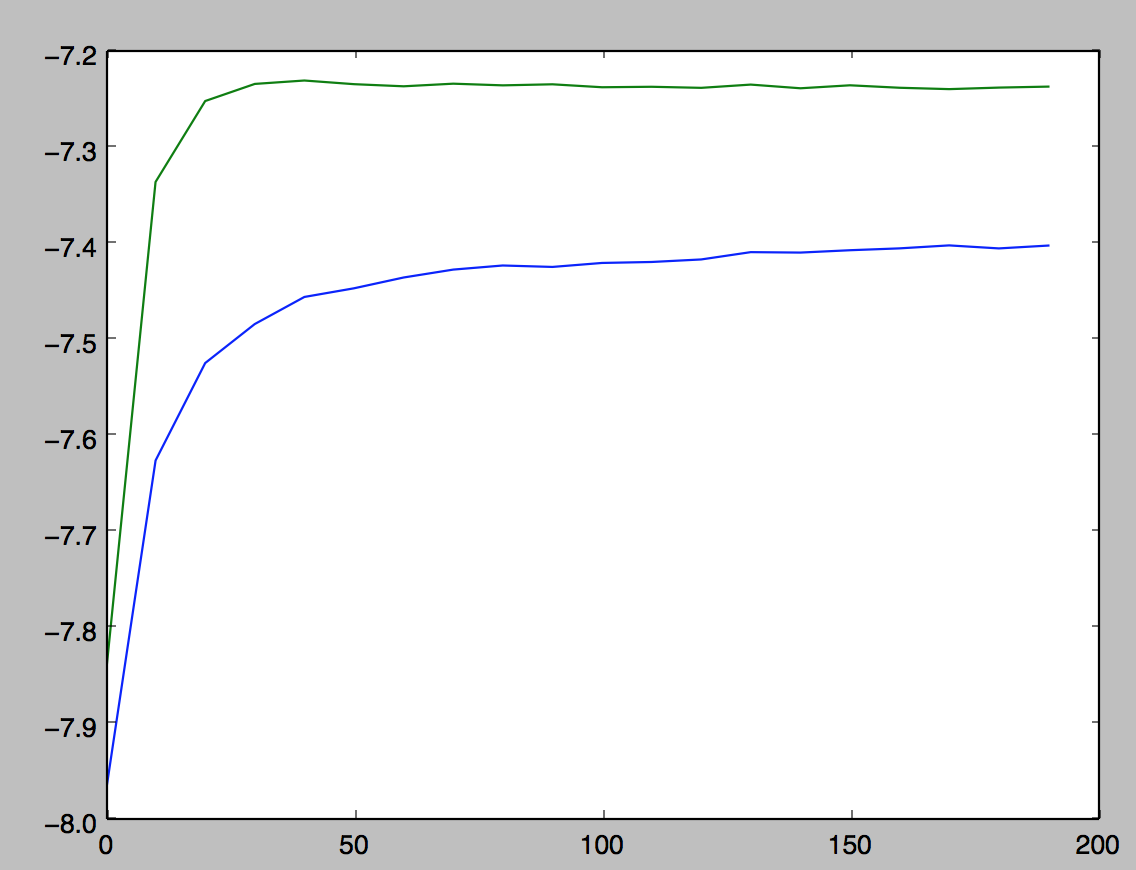
\includegraphics[width=6cm]{./pic/LLHW.png}
    \caption{Training LLHW}
\end{figure}

The green line is Upstream LDA and the bule is LDA.
We could see that the Neural Networks Upstream Conditioning LDA would achieve
higher training likelihood with faster speed. Therefore, it should be better
features that is more fitting to the data.

\subsubsection{Deep Learning Word Features}
I used the word2vec to get the Deep Learning Word Features
\cite{mikolov2013distributed}. Word2vec is famous for finding the most similar
word phrases. Here, I presented several typical similar words with cosine
similarity.


\begin{minipage}{.310\textwidth}
\centering
\textbf{Algorithm} \\
algorithms \quad 0.732173 \\
pruning \quad 0.715835 \\
method \quad 0.705341 \\
greedy \quad 0.700185 \\
heuristic \quad 0.692098\\
proposed \quad 0.687952 \\
technique \quad 0.666948 \\
iteratively \quad 0.616023 \\
tabu \quad 0.610261 \\
bisection \quad 0.607905
\end{minipage}
\begin{minipage}{.310\textwidth}
\centering
\textbf{Network} \\
networks \quad 0.825327 \\
topology \quad 0.744842 \\
wireless \quad 0.665959 \\
gateways \quad 0.657244 \\
link \quad 0.652112 \\
node \quad 0.541835 \\
topologies \quad 0.645444 \\
traffic \quad 0.639832 \\
nodes \quad 0.624277 \\
overlap \quad 0.607500
\end{minipage}
\begin{minipage}{.310\textwidth}
\centering
\textbf{Model} \\
models \quad 0.751951\\
modeling \quad 0656805\\
mathematic \quad 0.625505 \\
markov \quad 0.603707 \\
stoachastic \quad 0.603393\\
svm \quad 0.595648 \\
probabilistic \quad 0.5758 \\
lingo \quad 0.573474 \\
tree \quad 0.573412 \\
parametric \quad 0.573359
\end{minipage}

For our prediction goal, I used the doc2vec, a variant of word2vec, which could
transfer a doc to a numeric vector as our deep learning word features.

\subsection{Classification Performances}
After extracting features, we could start testing with classifiers to get the
classification performances.

First I just started with baseline methods. For baseline, I would use Scalable
Smoothed Naive Bayes, C4.5 Decision Trees, SVM implemented via SMO, and Two
Layer Neural Networks. For Naive Bayes, I used the basic word feature. For
other classifiers, I used the basic LDA topic distributions.


\begin{table}[h]
\renewcommand{\arraystretch}{1.5}
\centering
\begin{tabular}{|c|c|c|c|c|}
\hline
accuracy
& Naive Bayes
& Decision Tree
& SVM
& Neural Network \\
\hline
Training
& 0.556
& 0.633
& 0.626
& \textbf{0.643}\\
\hline
Tesing
& 0.515
& 0.605
& 0.634
& \textbf{0.645}\\
\hline
\end{tabular}
\caption{Baseline Methods with Basic Features}
\end{table}

From the above baseline method performance table, we could see with the basic
features, Naive Bayes is obviously worse than other classification methods.
Therefore, we no longer consider Naive Bayes for this task. Then I would
explored which feature would help most for prediction goal.

\begin{table}[h]
\renewcommand{\arraystretch}{1.5}
\centering
\begin{tabular}{|c|c|c|c|c|}
\hline
accuracy
& LDA
& Upstream LDA
& word2vec
& word2vec+UpLDA \\
\hline
DT
& 0.605
& 0.616
& 0.625
& 0.595\\
\hline
SVM
& 0.634
& 0.647
& \textbf{0.682}
& 0.685 \\
\hline
NN
& \textbf{0.643}
& \textbf{0.655}
& 0.678
& \textbf{0.707} \\
\hline
\end{tabular}
\caption{Test Performances with Different Features}
\end{table}

The results are showed in the table 2, which recorded the test performances for
each classifiers. From the table, we would know that in most cases, NN would be
the best choice for prediction goal. Besides, we would find that the best
feature is to combine Neural Networks Upstream Conditoning LDA feature, which are
trained with meta-data beyond basic topic distributions, and Deep Learning Word
Features, the word2vec. Another interesting fact is when combining UpLDA and
word2vec as feature, Decision Trees would get lower performances. This could be
that Decision Trees are always not scalable and tend to be overfitting with
large scale feature vector.

\subsection{Parameter Tuning for Optimization}
After finding the best classifier and best feature, then I do parameter tuning
for optimization. The basic parameter for NN is the number of hidden points in
the hidden layers. Basically, the more hidden points, the complex the model is.
For my Neural Networks, there are two layer, the second layer size was set to
10, which is the label size. So I tuned the first hidden number, ranging from
100 to 500, and got the results.


\begin{figure}[!htbp]
    \centering
    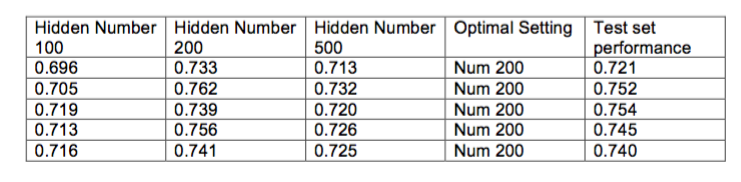
\includegraphics[width=14cm]{./pic/Result.png}
    \caption{Parameter Tuning}
\end{figure}

From the figure above, we would see that the Hidden Number = 200 would get the
best performances. Setting Hidden Number = 500 would be overfitting, which means
we are trying to use a too complex model to fit a comparatively simple dataset.

